\subsection{Forretningsmodel}
\label{section:forretningsmodel}

Psykolog Nord tilbyder psykologbehandling uden ventetid.
Derfor har de åbent alle 7 dage i ugen fra kl. 9 til 21.

Psykolog Nord er en psykologkæde med 3 afdelinger:
\begin{itemize}
    \item Aalborg
    \item Aarhus
    \item Odense
\end{itemize}

De har 3 psykologer:

\begin{itemize}
    \item Katrine Breum Larsen
    \item Miriam Poulsen
    \item Stefan Guldager Boldemann
\end{itemize}

Lige nu er Katrine og Miriam begge tilknyttet afdelingerne i Aalborg og Aarhus, og Stefan er tilknyttet afdelingen i Odense.


Firmaet drives af brødrene Anders Mikkelsen og Lasse Kirk, og Lasses kæreste Katrine Breum Larsen.
De har en flad firmastruktur, hvor alle 3 indgår i firmaets ledelse, men Katrine står for den daglige ledelse. 
Firmaet tilhører den basale form fra Mintzbergs fem organisationsformer, og på 
figur \ref{forretning:organisationsdiagram} kan man se deres virksomhedsstruktur.

De tilknyttede psykologer er ikke ansat af Psykolog Nord, men er partnere.
Derfor skal de ikke betale løn og pension, men derimod har de aftalt, at psykologen modtager halvdelen af betalingen fra klienten.
Deres indkomst er betalinger af fakturaer fra klienter.

Hvad laves der af markedsføring? De har en hjemmeside og en Facebook.

Deres kontakt med klienter er personlig, da du har en tilknyttet psykolog, som 
du har samtaler med. En oversigt over deres forretningsmodel kan ses på figur \ref{forretning:fml}.

\begin{figure}
    \caption{Organisationsdiagram for Psykolog Nord}
    \centering
        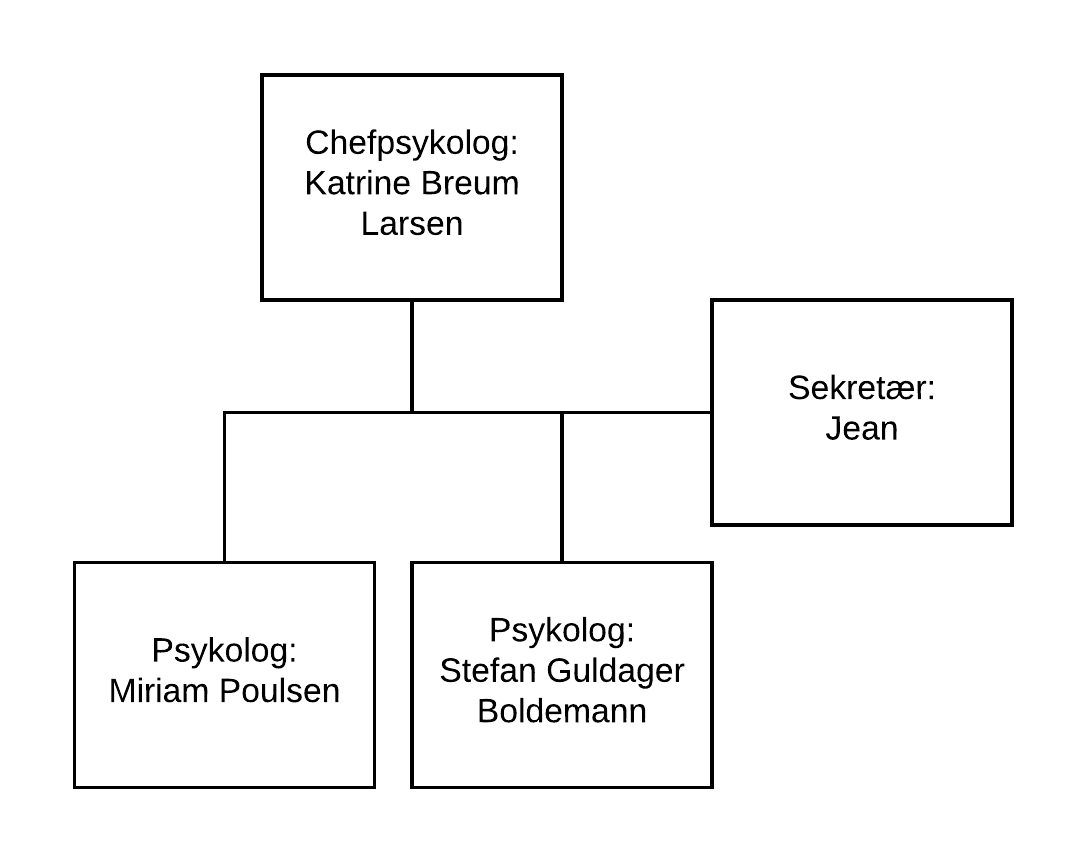
\includegraphics[scale=.8]{OrganisationsDiagram}
    \label{forretning:organisationsdiagram}
\end{figure}

\begin{figure}
    \caption{FML for Psykolog Nord}
    \centering
        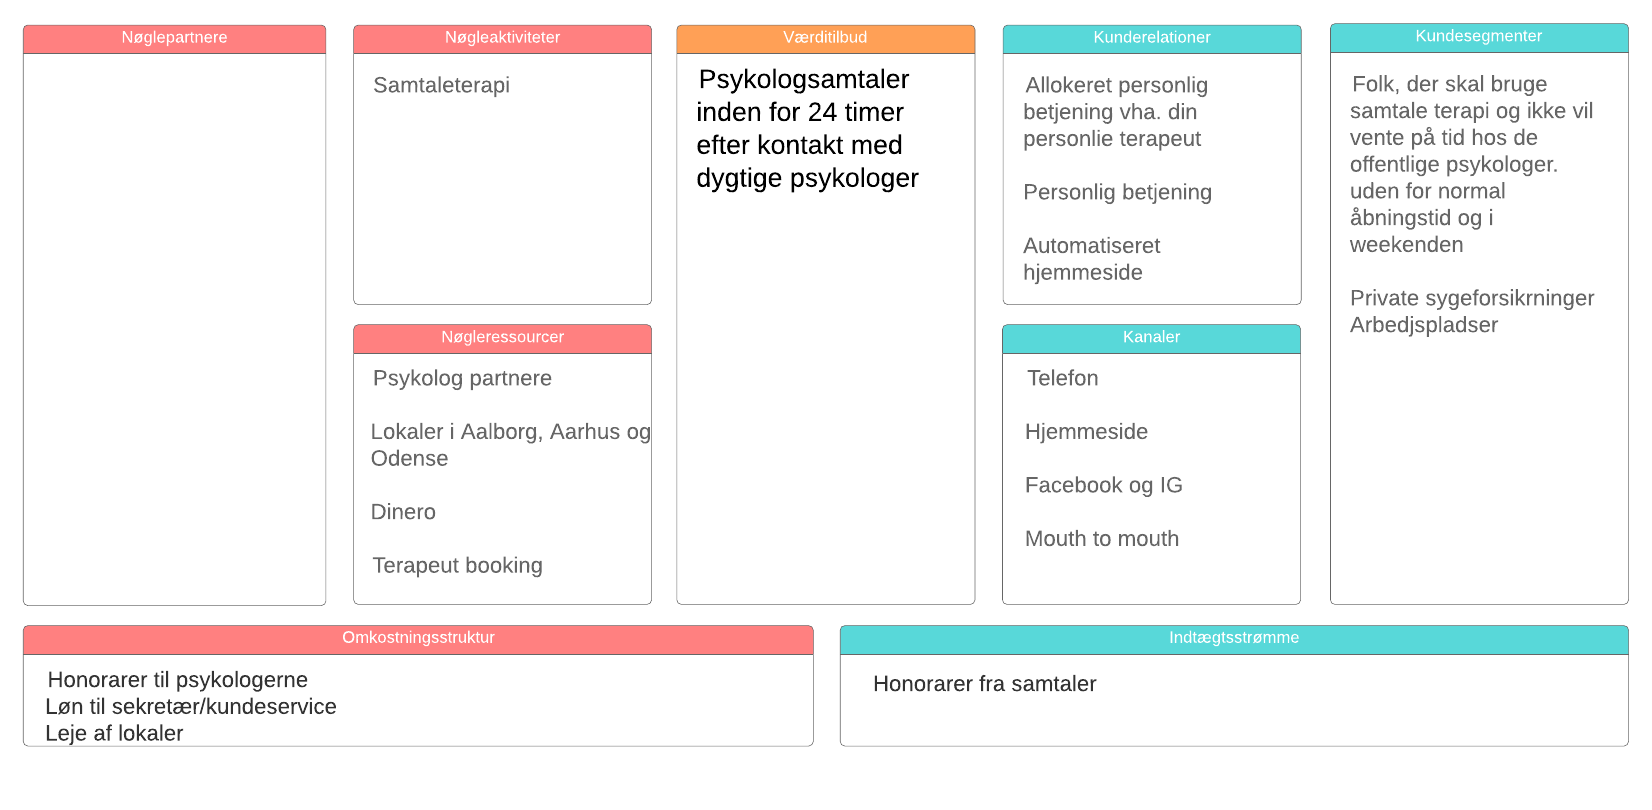
\includegraphics[width=\textwidth]{FML}
    \label{forretning:fml}
\end{figure}

